\chapter*{Введение. Обоснование актуальности} % * не проставляет номер
\addcontentsline{toc}{chapter}{ВВЕДЕНИЕ} % вносим в содержание

В большинстве современных компьютеров установлено и одновременно используются два вида вычислительных процессоров: центральный процессор (CPU) и графический (GPU). Из-за того что они работают одновременно, а также имеют обособленную друг от друга физическую память, возникает необходимость в синхронизации и передаче данных. Эту необходимость решает программа-драйвер, которую реализуют производители графических вычислительных процессоров, предоставляя разработчикам графических приложений специальные API, такие как OpenGL, Vulkan, DirectX 11 и тд. Однако, из-за того что заранее предугадать архитектурные особенности итоговых графических приложений невозможно, программа-драйвер может добавлять дополнительные синхронизации, что приводит к ухудшению производительности, так как центральный и графический процессоры начинают работать последовательно, как представлено на \firef{fig:pipeline_dx11}.

\begin{figure}[ht!] 
	\center
	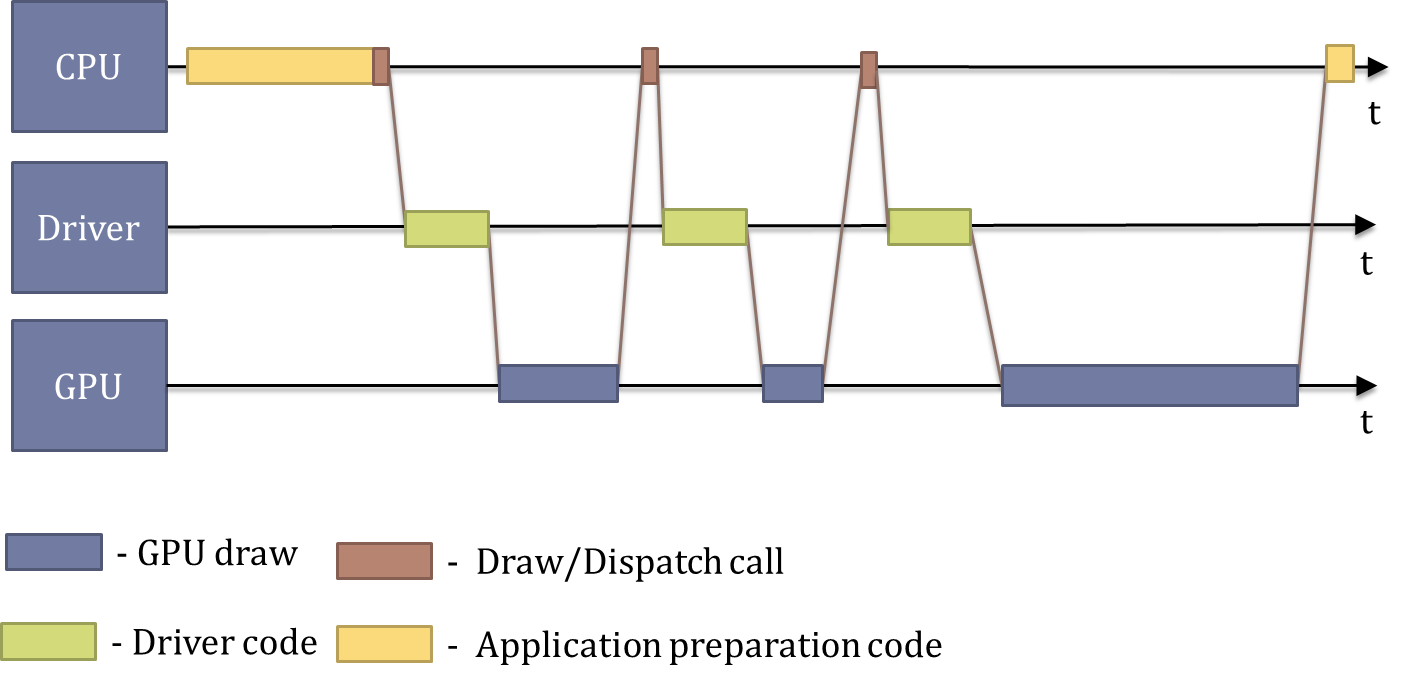
\includegraphics [scale=0.23] {my_folder/images//pipeline_dx11}
	\caption{Схема работы приложения при неоптимальном драйвере DirectX 11} 
	\label{fig:pipeline_dx11}  
\end{figure}

Во избежание подобных ситуаций, в более поздних и новых API (таких как DirectX 12 и Vukan) задача синхронизации была снята с программы драйвера и была передана разработчику. Для этого было введено понятие \say{списка команд}, который разработчик мог заполнять и затем отправлять на исполнение, как показано на \firef{fig:pipeline_dx12}.

\begin{figure}[ht!] 
	\center
	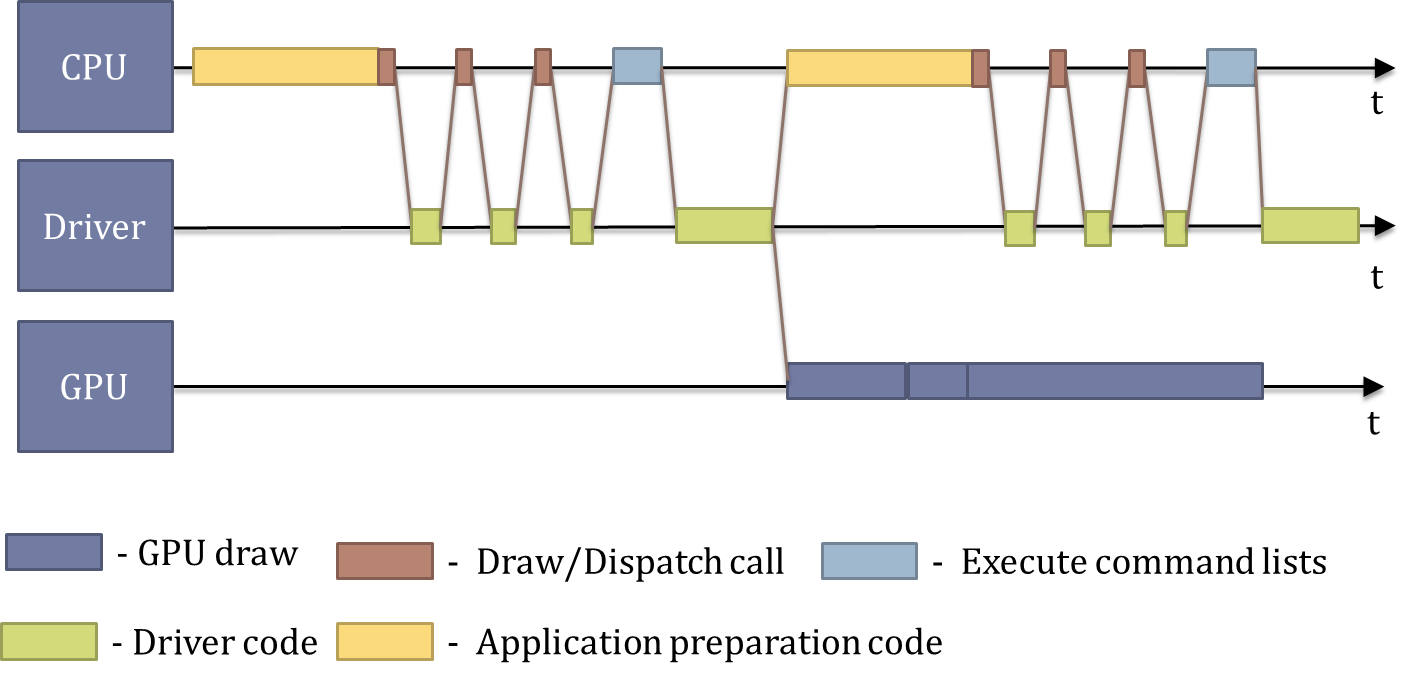
\includegraphics [scale=0.23] {my_folder/images//pipeline_dx12}
	\caption{Схема работы приложения при DirectX 12} 
	\label{fig:pipeline_dx12}  
\end{figure}

Однако несмотря на то, что данный подход даёт возможность явно управлять синхронизациями между процессорами, часть времени центрального процессора уходит на построение вышеупомянутого \say{списка}. Причём время построения и передачи будет зависеть от количества выводимых объектов (см. \firef{fig:pipeline_dx12_circles}).

\begin{figure}[ht!] 
	\center
	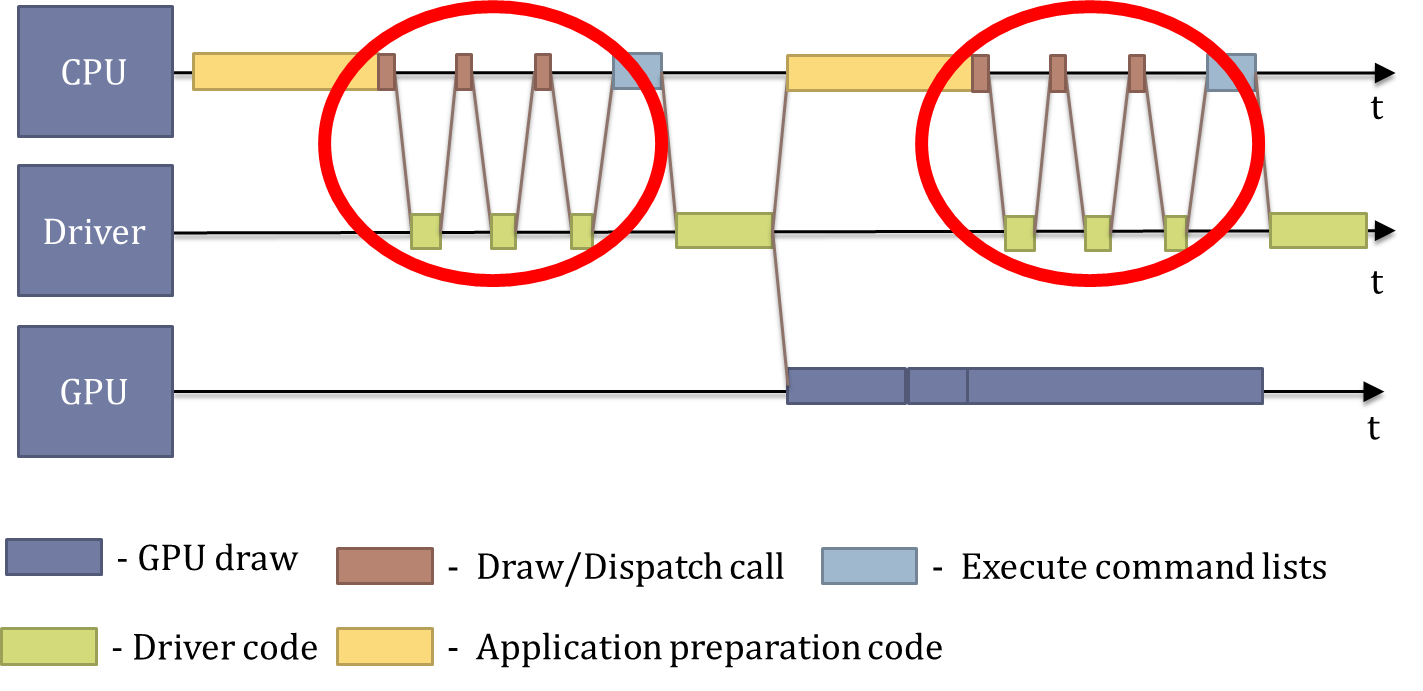
\includegraphics [scale=0.23] {my_folder/images//pipeline_dx12_circles}
	\caption{Схема работы приложения при DirectX 12, с выделенным временем на построение списка выводимых объектов} 
	\label{fig:pipeline_dx12_circles}  
\end{figure}

Целью работы является построение архитектуры графического приложения таким образом, чтобы время построения и передачи, а также размер \say{списка команд} не зависели от количества выводимых объектов (см. \firef{fig:pipeline_dx12_me}). Таким образом разработчику ПО будет предоставлено больше времени центрального процессора, а значит более трудоёмкие алгоритмы можно будет использовать для достижения желаемых результатов.

\begin{figure}[ht!] 
	\center
	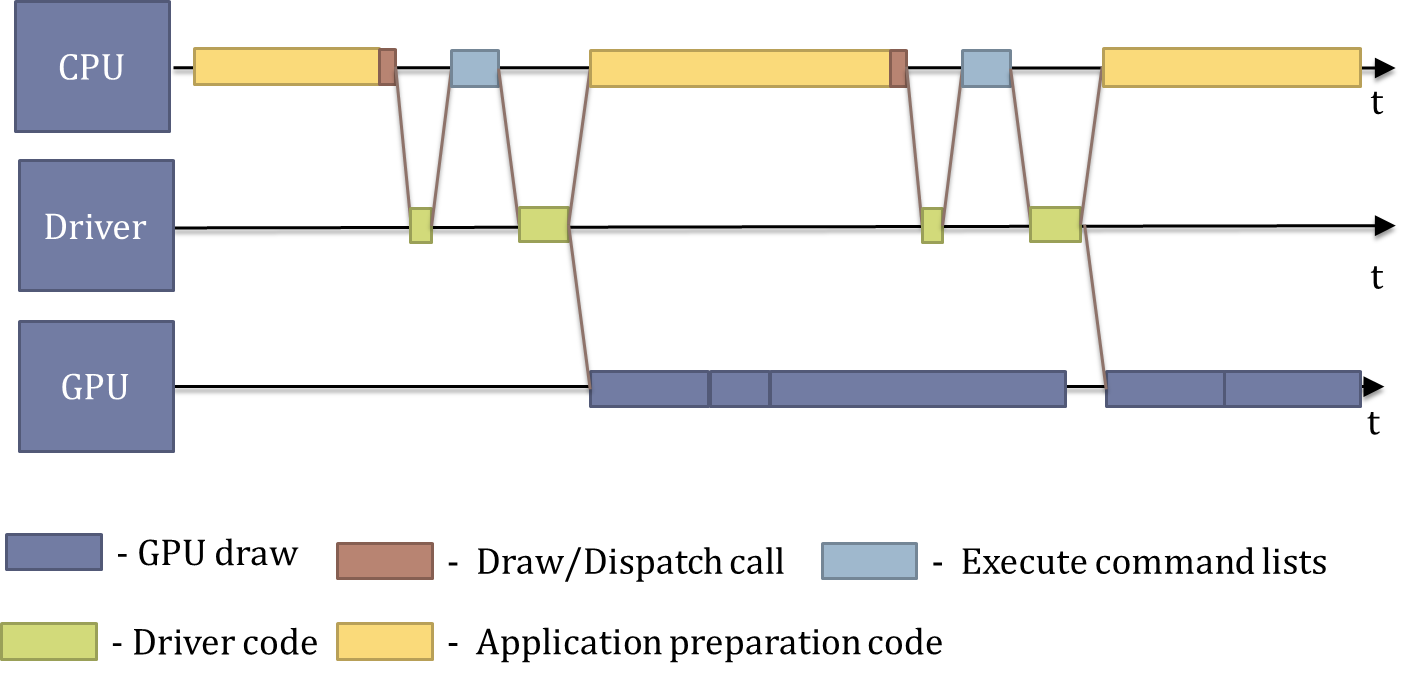
\includegraphics [scale=0.23] {my_folder/images//pipeline_dx12_me}
	\caption{Схема работы приложения при DirectX 12 с использованием предлагаемого конвейера} 
	\label{fig:pipeline_dx12_me}  
\end{figure}

%% Вспомогательные команды - Additional commands
%\newpage % принудительное начало с новой страницы, использовать только в конце раздела
%\clearpage % осуществляется пакетом <<placeins>> в пределах секций
%\newpage\leavevmode\thispagestyle{empty}\newpage % 100 % начало новой строки